\section{Анализ автоматизируемого бизнес-процесса}\label{sec:business-process-analysis}

\subsection{Построение модели AS-IS}\label{subsec:business-process-as-is-modeling}

С точки зрения организации-исполнителя автоматизируемый бизнес-процесс разработки отдельного веб-сервиса в модели AS-IS включает в себя следующие этапы:

\begin{enumerate}
	\item Заказчик находит дефект или неточность в работе веб-сервиса и сообщает об этом руководителю проекта.
	\item Руководитель проекта анализирует полученную от заказчика обратную связь и создаёт задачу в трекере.
	\item Руководитель команды знакомится с поставленной задачей в трекере, определяет сложность и риски. Если выполнение задачи подразумевает существенные ограничения, то заказчик информируется о невозможности реализации.
	\item Руководитель команды назначает ответственных за выполнение задачи.
	\item Поставленный разработчик вносит изменения в исходный код веб-сервиса и отправляет результат во временную ветку удалённого репозитория.
	\item Руководитель команды производит ручное тестирование веб-сервиса, проверяет качество кода в ветке удалённого репозитория и даёт обратную связь. Если по задаче возникают замечания, то она отправляется на доработку.
	\item Руководитель команды сливает исходный код в основную ветку удалённого репозитория.
	\item Системный администратор производит ручную сборку исходного кода веб-сервиса и запускает полученный артефакт в staging-среде.
	\item Руководитель проекта тестирует изменения на staging-сервере. Если по задаче возникают замечания, то она отправляется на доработку.
	\item Руководитель проекта демонстрирует изменения заказчику. Если по задаче возникают замечания, то она отправляется на доработку.
	\item Системный администратор производит ручную сборку исходного кода веб-сервиса и запускает полученный артефакт в production-среде.
	\item Заказчик подтверждает руководителю проекта тот факт, что дефект или неточность в работе веб-сервиса была исправлена.
\end{enumerate}

\subsection{Бизнес-процесс в модели TO-BE}\label{subsec:business-process-in-to-be-model}

В отличие от первой версии бизнес-процесса, операции по доставке изменённых веб-сервисов в целевые среды выполняет подсистема автоматизации сборки и развёртывания.\ При этом первичный анализ рисков, постановка задачи, проверка исходного кода и согласование реализованного функционала остаются в зоне ответственности каждого из участников процесса.

Отправка изменений во временную ветку автоматически запускает сборку изменённых веб-сервисов и развёртывание отдельного экземпляра приложения в тестовой среде.\ Если в ходе сборки или развёртывания возникают ошибки, разработчик получает информацию о них и вносит необходимые исправления, после чего повторная отправка изменений запускает эти операции заново.

Проверка исходного кода на соответствие техническому заданию в таком варианте бизнес-процесса существенно упрощается, поскольку работающий экземпляр уже собран и позволяет наглядно протестировать изменения. Кроме того, автоматическое развёртывание по мере слияний в основную ветку позволяет добиться постоянной синхронизации между актуальным исходным кодом и пре-продакшеном.

После выполнения всех требований заказчика руководитель команды в соответствии с установленным расписанием релизов самостоятельно инициирует развёртывание согласованной версии приложения в продакшен через интерфейс подсистемы автоматизации.

Модель бизнес-процесса после внедрения автоматизации представлена на рисунке~\ref{fig:business-process-to-be}. Состав поставщиков, входов, основных процессов, выходов и потребителей модели TO-BE представлен в таблице~\ref{tab:sipoc-to-be} по методологии SIPOC.

\begin{landscape}
	\begin{table}[p]
		\centering
		\caption{SIPOC-модель бизнес-процесса TO-BE}\label{tab:sipoc-to-be}
		\footnotesize
		\setstretch{1}
		\setlength{\tabcolsep}{5pt}
		\renewcommand{\arraystretch}{1.15}
		\begin{tabularx}{\linewidth}{|Y{0.9}|Y{0.95}|Y{1.3}|Y{1.05}|Y{0.8}|}
			\hline
			\textbf{Поставщики} & \textbf{Входы} & \textbf{Процессы} & \textbf{Выходы} & \textbf{Потребители} \\
			\hline
			Заказчик; менеджер проекта &
			Обратная связь: функциональная проблема или дефект &
			1. Первичный анализ рисков, ограничений и возможности реализации руководителем команды &
			Решение о согласовании изменения или отказе от его реализации &
			Руководитель команды \\
			\hline
			Руководитель команды &
			Согласованное изменение; выявленные ограничения &
			2. Подготовка технического задания, создание задачи в трекере и назначение разработчиков &
			Техническое задание; задача с назначенными исполнителями &
			Разработчик \\
			\hline
			Руководитель команды; разработчик &
			Техническое задание; исходный код компонентов системы &
			3. Внесение изменений и отправка кода во временную ветку репозитория &
			Изменённый код; событие отправки изменений в ветку &
			Подсистема автоматизации \\
			\hline
			Разработчик &
			Код временной ветки; событие её обновления &
			4. Автоматическая сборка и развёртывание тестового экземпляра при обновлении ветки &
			Тестовый экземпляр либо сообщение об ошибках сборки и развёртывания &
			Руководитель команды; разработчик \\
			\hline
			Руководитель команды; разработчик; подсистема автоматизации &
			Техническое задание; исходный код; работающий тестовый экземпляр &
			5. Проверка кода и тестирование руководителем; слияние изменений в основную ветку &
			Проверенный код в основной ветке либо замечания для доработки &
			Подсистема автоматизации; разработчик \\
			\hline
			Руководитель команды; заказчик &
			Код основной ветки; событие слияния; требования заказчика &
			6. Автоматическая сборка и развёртывание в пре-продакшене; проверка и согласование заказчиком &
			Экземпляр в пре-продакшене; согласование изменений либо замечания &
			Заказчик; руководитель команды; разработчик \\
			\hline
			Заказчик; руководитель команды &
			Согласованная версия приложения; команда на выпуск по расписанию релизов &
			7. Запуск выпуска руководителем через интерфейс подсистемы; автоматическое развёртывание в продакшене &
			Обновлённая система в рабочей среде &
			Заказчик; пользователи системы \\
			\hline
		\end{tabularx}
	\end{table}
\end{landscape}


\begin{landscape}
	\begin{table}[p]
		\centering
		\caption{SIPOC-модель бизнес-процесса AS-IS}\label{tab:sipoc-as-is}
		\footnotesize
		\setstretch{1}
		\setlength{\tabcolsep}{5pt}
		\renewcommand{\arraystretch}{1.15}
		\begin{tabularx}{\linewidth}{|Y{0.9}|Y{0.95}|Y{1.3}|Y{1.05}|Y{0.8}|}
			\hline
			\textbf{Поставщики} & \textbf{Входы} & \textbf{Процессы} & \textbf{Выходы} & \textbf{Потребители} \\
			\hline
			Заказчик; менеджер проекта &
			Обратная связь: функциональная проблема или дефект &
			1. Первичный анализ рисков, ограничений и возможности реализации руководителем команды &
			Решение о согласовании изменения или отказе от его реализации &
			Руководитель команды \\
			\hline
			Руководитель команды &
			Согласованное изменение; выявленные ограничения &
			2. Подготовка технического задания, создание задачи в трекере и назначение разработчиков &
			Техническое задание; задача с назначенными исполнителями &
			Разработчик \\
			\hline
			Руководитель команды; разработчик &
			Техническое задание; исходный код компонентов системы &
			3. Внесение изменений и отправка кода во временную ветку репозитория &
			Изменённый исходный код во временной ветке &
			Руководитель команды \\
			\hline
			Разработчик; руководитель команды &
			Код временной ветки; техническое задание &
			4. Проверка кода руководителем; ручная сборка и развёртывание в тестовой среде администратором &
			Согласованный код и тестовый экземпляр либо замечания по коду &
			Руководитель команды; разработчик \\
			\hline
			Системный администратор; руководитель команды &
			Тестовый экземпляр; согласованный исходный код &
			5. Тестирование функционала и совместимости; слияние в основную ветку руководителем команды &
			Проверенный код в основной ветке либо сведения о дефектах &
			Системный администратор; разработчик \\
			\hline
			Руководитель команды; заказчик &
			Код основной ветки; требования заказчика &
			6. Ручная сборка и развёртывание в пре-продакшене; проверка и согласование заказчиком &
			Экземпляр в пре-продакшене; согласование изменений либо замечания &
			Заказчик; системный администратор; разработчик \\
			\hline
			Заказчик; руководитель команды &
			Подтверждение выполнения требований; согласованная версия исходного кода &
			7. Ручная сборка и выпуск системы в продакшен системным администратором &
			Обновлённая система в рабочей среде &
			Заказчик; пользователи системы \\
			\hline
		\end{tabularx}
	\end{table}
\end{landscape}

\begin{landscape}
	\begin{table}[p]
		\centering
		\caption{SIPOC-модель бизнес-процесса TO-BE}\label{tab:sipoc-to-be}
		\footnotesize
		\setstretch{1}
		\setlength{\tabcolsep}{5pt}
		\renewcommand{\arraystretch}{1.15}
		\begin{tabularx}{\linewidth}{|Y{0.9}|Y{0.95}|Y{1.3}|Y{1.05}|Y{0.8}|}
			\hline
			\textbf{Поставщики} & \textbf{Входы} & \textbf{Процессы} & \textbf{Выходы} & \textbf{Потребители} \\
			\hline
			Заказчик; менеджер проекта &
			Обратная связь: функциональная проблема или дефект &
			1. Первичный анализ рисков, ограничений и возможности реализации руководителем команды &
			Решение о согласовании изменения или отказе от его реализации &
			Руководитель команды \\
			\hline
			Руководитель команды &
			Согласованное изменение; выявленные ограничения &
			2. Подготовка технического задания, создание задачи в трекере и назначение разработчиков &
			Техническое задание; задача с назначенными исполнителями &
			Разработчик \\
			\hline
			Руководитель команды; разработчик &
			Техническое задание; исходный код компонентов системы &
			3. Внесение изменений и отправка кода во временную ветку репозитория &
			Изменённый код; событие отправки изменений в ветку &
			Подсистема автоматизации \\
			\hline
			Разработчик &
			Код временной ветки; событие её обновления &
			4. Автоматическая сборка и развёртывание тестового экземпляра при обновлении ветки &
			Тестовый экземпляр либо сообщение об ошибках сборки и развёртывания &
			Руководитель команды; разработчик \\
			\hline
			Руководитель команды; разработчик; подсистема автоматизации &
			Техническое задание; исходный код; работающий тестовый экземпляр &
			5. Проверка кода и тестирование руководителем; слияние изменений в основную ветку &
			Проверенный код в основной ветке либо замечания для доработки &
			Подсистема автоматизации; разработчик \\
			\hline
			Руководитель команды; заказчик &
			Код основной ветки; событие слияния; требования заказчика &
			6. Автоматическая сборка и развёртывание в пре-продакшене; проверка и согласование заказчиком &
			Экземпляр в пре-продакшене; согласование изменений либо замечания &
			Заказчик; руководитель команды; разработчик \\
			\hline
			Заказчик; руководитель команды &
			Согласованная версия приложения; команда на выпуск по расписанию релизов &
			7. Запуск выпуска руководителем через интерфейс подсистемы; автоматическое развёртывание в продакшене &
			Обновлённая система в рабочей среде &
			Заказчик; пользователи системы \\
			\hline
		\end{tabularx}
	\end{table}
\end{landscape}

\begin{landscape}
	\begin{figure}[p]
		\centering
		\begin{minipage}{0.86\linewidth}
			\centering
			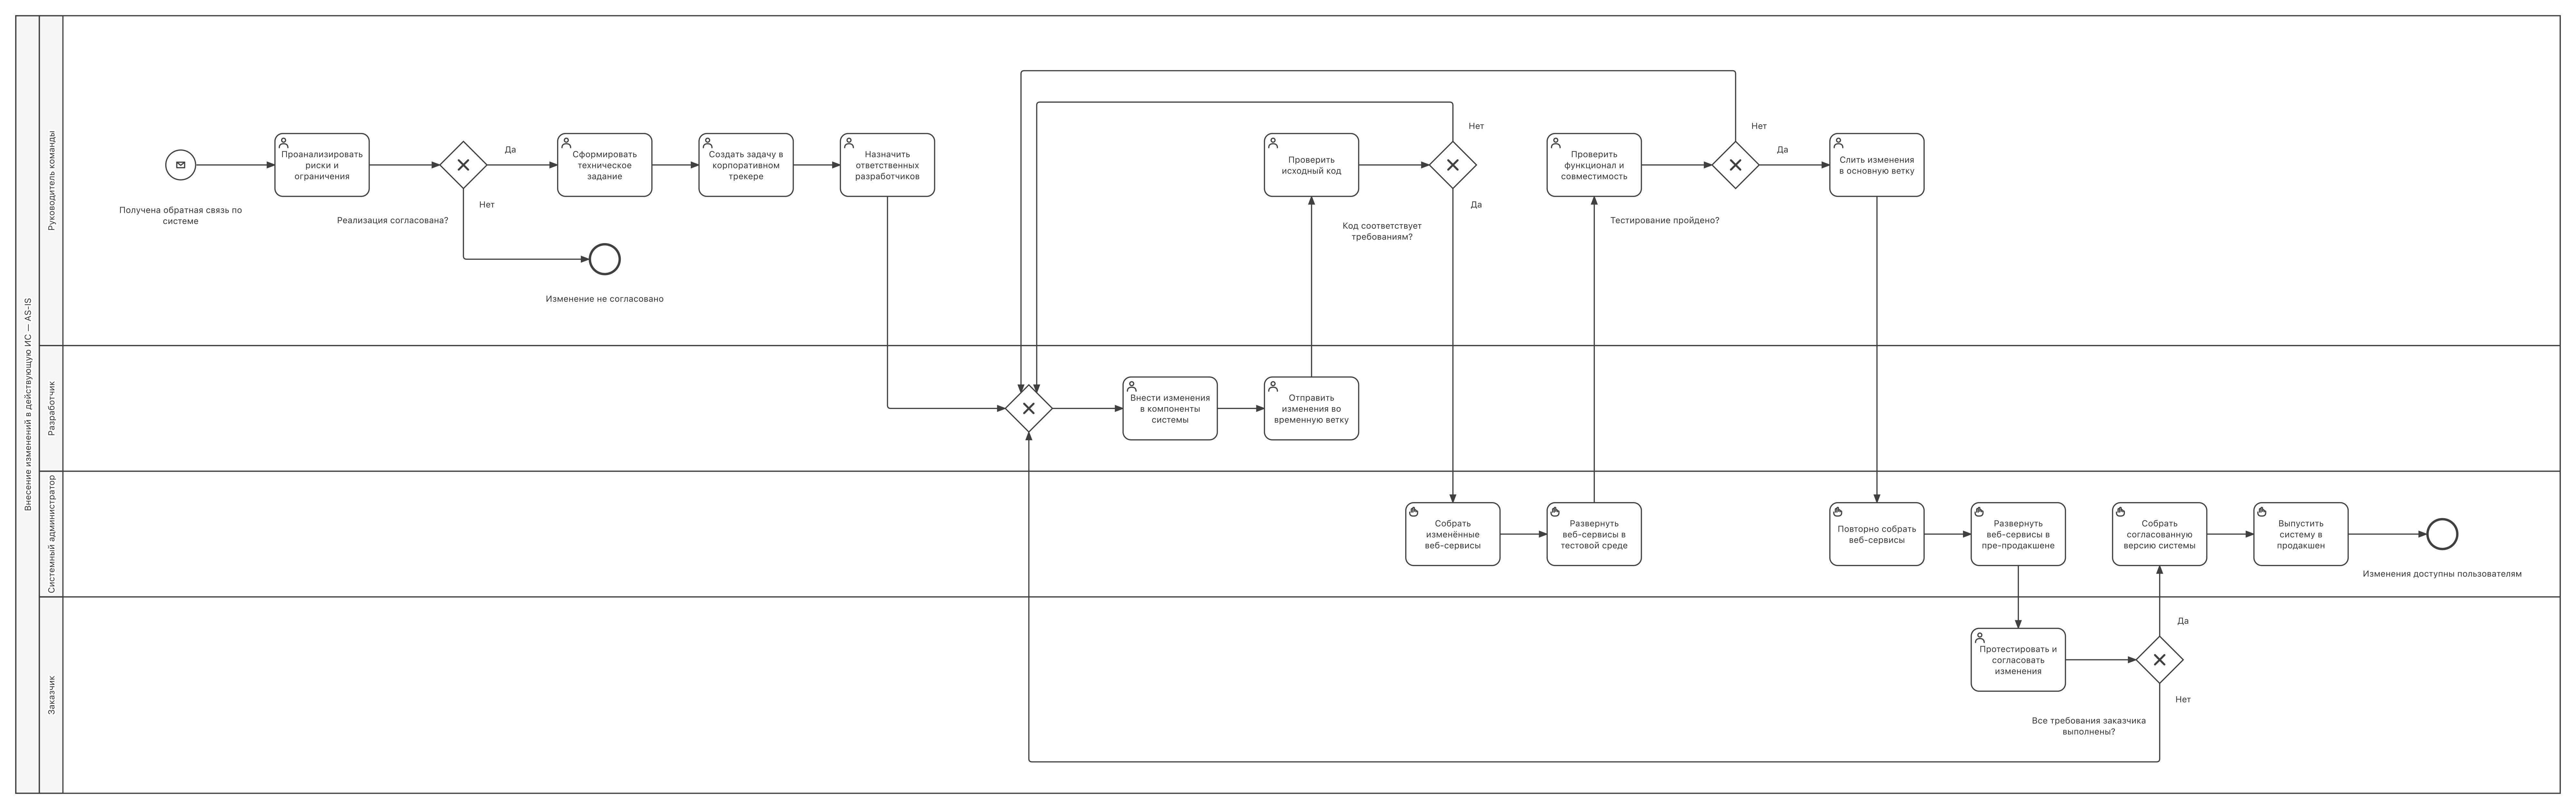
\includegraphics[width=\linewidth]{bpmn-as-is}
			\caption{Модель AS-IS процесса внесения изменений}\label{fig:business-process-as-is}

			\medskip

			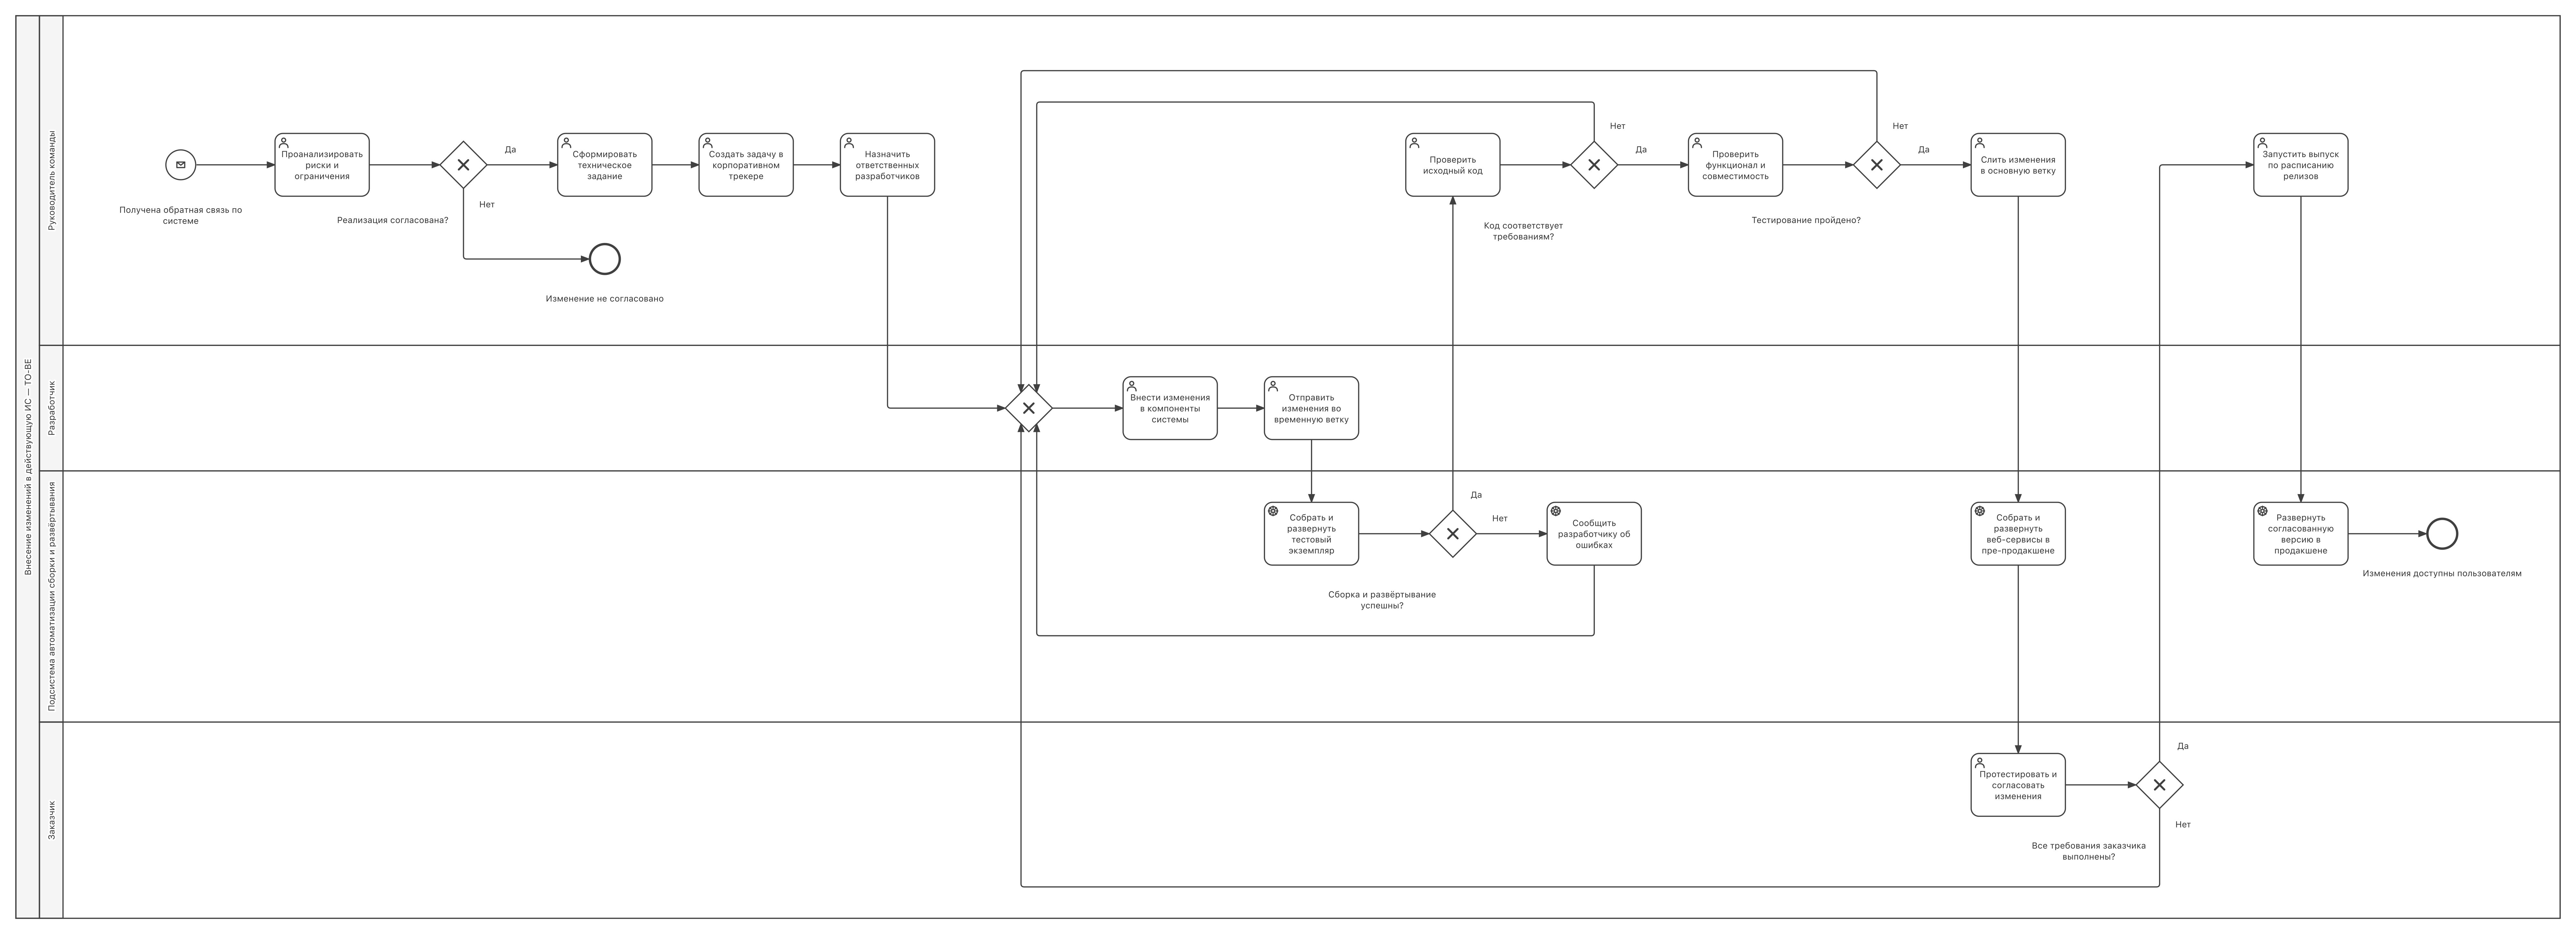
\includegraphics[width=\linewidth]{bpmn-to-be}
			\caption{Модель TO-BE процесса внесения изменений}\label{fig:business-process-to-be}
		\end{minipage}
	\end{figure}
\end{landscape}
